% Copyright 2004 by Till Tantau <tantau@users.sourceforge.net>.
%
% In principle, this file can be redistributed and/or modified under
% the terms of the GNU Public License, version 2.
%
% However, this file is supposed to be a template to be modified
% for your own needs. For this reason, if you use this file as a
% template and not specifically distribute it as part of a another
% package/program, I grant the extra permission to freely copy and
% modify this file as you see fit and even to delete this copyright
% notice. 
\UseRawInputEncoding
\documentclass{beamer}

% There are many different themes available for Beamer. A comprehensive
% list with examples is given here:
% http://deic.uab.es/~iblanes/beamer_gallery/index_by_theme.html
% You can uncomment the themes below if you would like to use a different
% one:
%\usetheme{AnnArbor}
%\usetheme{Antibes}
%\usetheme{Bergen}
%\usetheme{Berkeley}
%\usetheme{Berlin}
%\usetheme{Boadilla}
%\usetheme{boxes}
%\usetheme{CambridgeUS}
%\usetheme{Copenhagen}
%\usetheme{Darmstadt}
%\usetheme{default}
%\usetheme{Frankfurt}
%\usetheme{Goettingen}
%\usetheme{Hannover}
%\usetheme{Ilmenau}
%\usetheme{JuanLesPins}
%\usetheme{Luebeck}
\usetheme{Madrid}
%\usetheme{Malmoe}
%\usetheme{Marburg}
%\usetheme{Montpellier}
%\usetheme{PaloAlto}
%\usetheme{Pittsburgh}
%\usetheme{Rochester}
%\usetheme{Singapore}
%\usetheme{Szeged}
%\usetheme{Warsaw}

\usepackage{pgfgantt}
%\usepackage{todonotes}
\usepackage{media9}
\usepackage{subfigure}


% Customize Warsaw color 
\setbeamercolor*{palette primary}{use=structure,fg=white,bg=red!50!black}
\setbeamercolor*{palette secondary}{use=structure,fg=white,bg=red!60!black}
\setbeamercolor*{palette tertiary}{use=structure,fg=white,bg=red!70!black}

% Customize Warsaw block title and background colors
\setbeamercolor{block title}{bg=red!50!black,fg=white}

\setbeamertemplate{bibliography item}{\insertbiblabel}  % insert bibliography numbers instead of symbol
\setbeamertemplate{caption}[numbered] % adds the figure or table number to the caption.



\title[2-DOF Helicopter (Proposal)]{Smart Control Algorithm for 2-DOF Helicopter}

% % A subtitle is optional and this may be deleted
% \subtitle{Product Proposal}

\author[G.~Janiak, K.~Vonckx]{Glenn~Janiak \and Kenneth~Vonckx \and
Advisor: Dr. Suruz Miah}
% - Give the names in the same order as the appear in the paper.
% - Use the \inst{?} command only if the authors have different
%   affiliation.

\institute[Bradley University] % (optional, but mostly needed)
{
  Department of Electrical and Computer Engineering\\
  Bradley University\\
  1501 W. Bradley Avenue\\
  Peoria, IL, 61625, USA
}
% - Use the \inst command only if there are several affiliations.
% - Keep it simple, no one is interested in your street address.

%\date[November~27,~2018]{Tuesday, November~27,~2018}
\date[November~29,~2018]{Thursday, November~29,~2018}
%\date[December~4,~2018]{Tuesday, December~4,~2016}

% - Either use conference name or its abbreviation.
% - Not really informative to the audience, more for people (including
%   yourself) who are reading the slides online

\logo{\hfill\href{http://www.bradley.edu}{
\includegraphics[width=0.75cm]{figs/logoBU1-Print}}}  % place logo in every page 

\subject{Mobile Robot Localization}
% This is only inserted into the PDF information catalog. Can be left
% out. 

% If you have a file called "university-logo-filename.xxx", where xxx
% is a graphic format that can be processed by latex or pdflatex,
% resp., then you can add a logo as follows:

% \pgfdeclareimage[height=0.5cm]{university-logo}{university-logo-filename}
% \logo{\pgfuseimage{university-logo}}

% Delete this, if you do not want the table of contents to pop up at
% the beginning of each subsection:
\AtBeginSubsection[]
{
  \begin{frame}<beamer>{Outline}
    \tableofcontents[currentsection,currentsubsection]
  \end{frame}
}

% Let's get started
\begin{document}

\begin{frame}
  \titlepage
\end{frame}

\begin{frame}{Outline} %Glenn
  \tableofcontents%[pausesections]
  % You might wish to add the option [pausesections]
\end{frame}

% Section and subsections will appear in the presentation overview
% and table of contents.
\section{Introduction}

\begin{frame}{Introduction}{} %Ken
  % applications of mobile robot navigation and problem description
    \begin{itemize}
        \item Helicopter are important for short-distance travel
            \begin{itemize}
                \item air-sea rescue
                \item fire fighting
                \item traffic control
                \item tourism
            \end{itemize}
        \item Purpose of control system
            \begin{itemize}
                \item resistance to turbulence
                \item enable use of mobile device
            \end{itemize}
        \item Which is better?
            \begin{itemize}
                \item Fundamental (LQR)
                \item Noise Filtering (LQG) 
                \item Machine Learning (ADP)
            \end{itemize}
    \end{itemize}
\end{frame}

\begin{frame}{Introduction}{} %Glenn
\begin{figure}
  \centering
  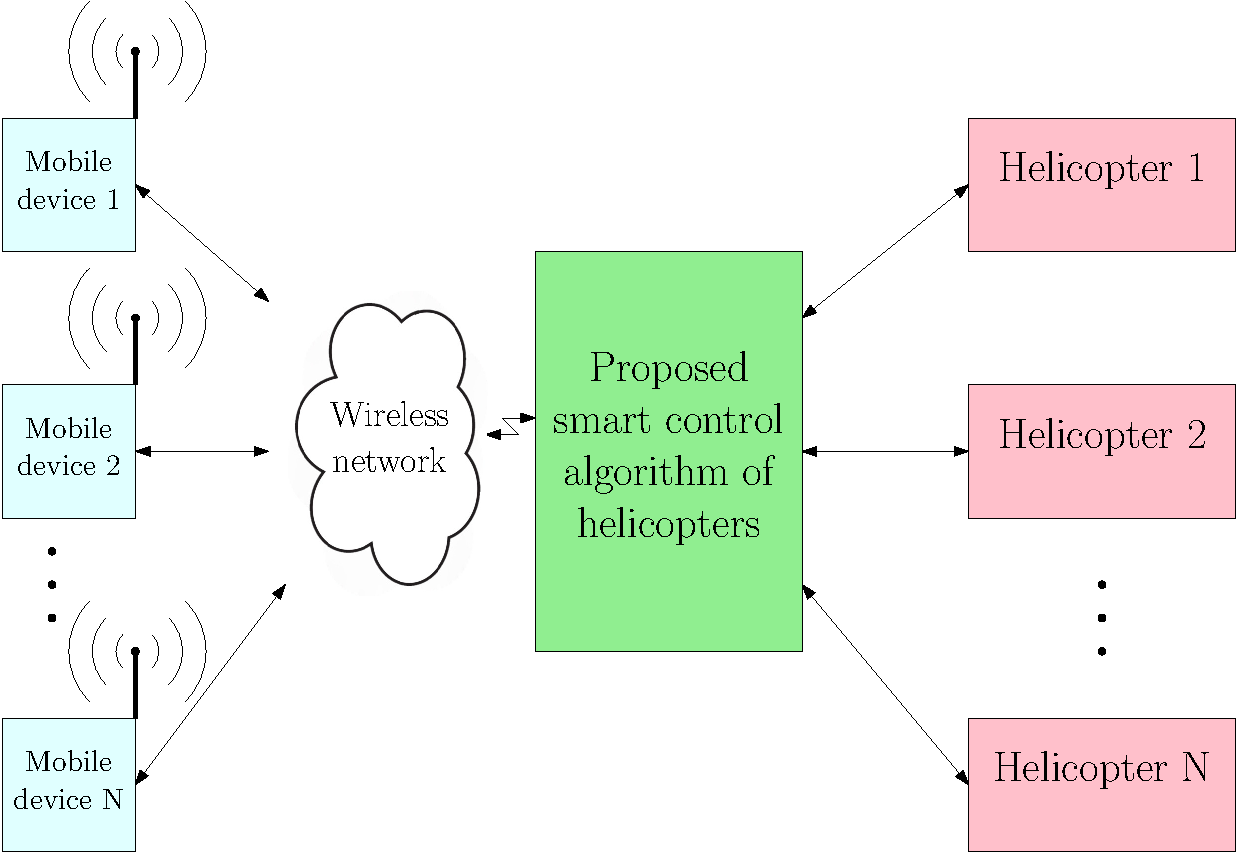
\includegraphics[scale=0.31]{figs/ipe/highLevel_wht_grn}
  \caption{General High-Level System Architecture}
  \label{fig:highLevel}
\end{figure}
\end{frame}

\begin{frame}{Introduction}{} %Glenn
        \begin{itemize}
        \item This project will:
            \begin{itemize}
                \item use a pair of 2-DOF (2-degrees-of-freedom) testing platforms
                \item implement control algorithms on embedded system
                \item use mobile device for user control
                \item encourage research
                \item serve as an educational tool
            \end{itemize}
        \end{itemize}
\end{frame}

%----------------------------------

\section{Background Study}
\subsection{Control Techniques}
\begin{frame}{Background Study}{Control Techniques} %Ken
    Various control techniques have been proposed for 2-DOF helicopters such as:
    \begin{itemize}
        \item Sliding mode control \cite{Ahmed2010-Sliding} %cite 2-Sliding Mode Based Robust Control for 2-DOF Helicopter here
        \item Fuzzy Logic control 
        \cite{Chang2017-Fuzzy}
        \cite{Kayacan2016-Fuzzy}
        \cite{Méndez-Monroy2012-Fuzzy} 
        %cite Fuzzy control with estimated variable sampling period for non-linear networked control systems: 2-DOF helicopter as case study here
        \item Data-driven Adaptive Optimal Output-feedback control \cite{Gao2016-DataDriven} %cite Data-driven Adaptive Optimal Output-feedback Control of a 2-DOF Helicopter here
        \item Decentralized discrete-time neural control \cite{Hernandez-Gonzalez2012-Decentralized} %cite Decentralized discrete-time neural control for a Quanser 2-DOF helicopter here
    \end{itemize}
    These control techniques employ advanced mathematics that are difficult to implement on embedded systems.
\end{frame}

%----------------------------------

\subsection{Modeling a 2-DOF Helicopter}

\begin{frame}{Background Study}{Modeling a 2-DOF Helicopter}
    \begin{columns}
    \column{0.5\textwidth}
    \begin{figure}
        \centering
        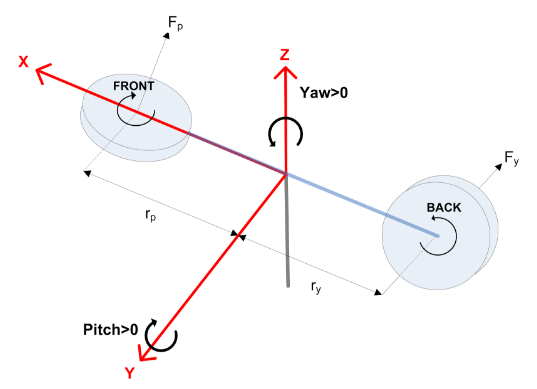
\includegraphics[width=\textwidth]{figs/img/helicopterModel}
        \caption{Model of a 2-DOF Helicopter}
        \label{fig:helicopterModel}
    \end{figure}
    \column{0.5\textwidth}
    \begin{figure}
      \centering 
      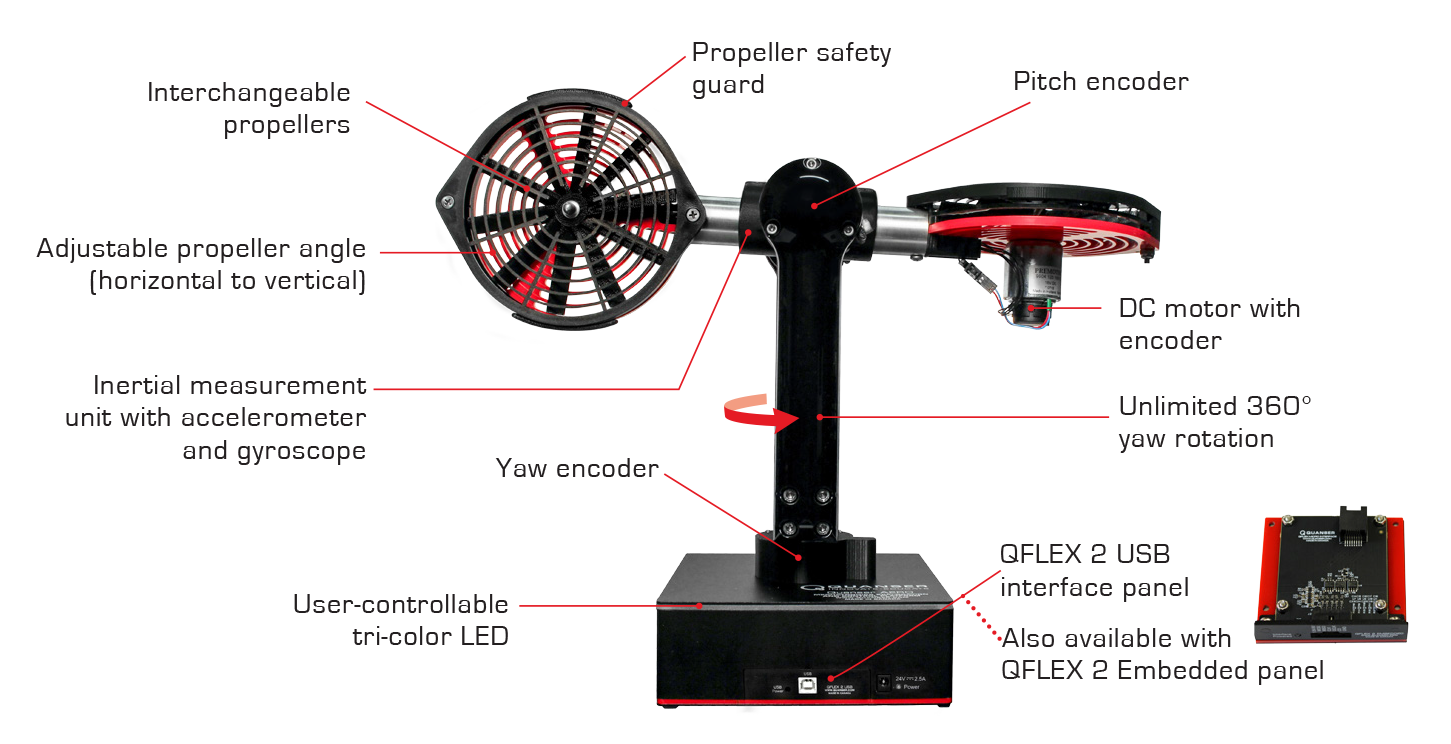
\includegraphics[width=\textwidth]{figs/img/quanserAero}
      \caption{Quanser Aero}
      \label{fig:QuanserAero}
    \end{figure}    
    \end{columns}

\end{frame}

\begin{frame}{Background Study}{Modeling a 2-DOF Helicopter} %Ken
    \begin{itemize}
        \item Characterized by fixed base
        \begin{itemize}
            \item Can change 2 of 3 possible orientations...
            \begin{itemize}
                \item Pitch ($\theta$)
                \item Yaw ($\psi$)
                \item \emph{Not Roll}
            \end{itemize}
            \item and cannot change position
            \begin{itemize}
                \item x direction
                \item y direction
                \item z direction
            \end{itemize}
        \end{itemize} 
    \end{itemize}
\end{frame}

% \begin{frame}{Background Study}{Quanser Aero} %Glenn

% \end{frame}

\begin{frame}{Background Study}{Modeling a 2-DOF Helicopter}
    \begin{itemize}
        \item Motors are attached to the propellers to create thrust due to air resistance
            \begin{itemize}
                \item Main - changes pitch angle
                \item Tail - changes yaw angle
            \end{itemize} 
        \item Torque due to rotation also creates a force on opposite axes 
    \end{itemize}
\end{frame}

\begin{frame}{Background Study}{Modeling a 2-DOF Helicopter}
\begin{align}
  \dot{\bf x}(t) = {\bf A}{\bf x}(t) +{\bf B}{\bf u}(t),~\mathrm{where}
\label{eq:stateModel}
\end{align}  
%
\begin{align*}
{\bf A} =  
\begin{bmatrix}
0 & 0 & 1 & 0\\
0 & 0 & 0 & 1\\
-\frac{K_{\text{sp}}}{J_p} & 0 & -\frac{D_p}{J_p} &  0\\
0 & 0 & 0 & -\frac{D_y}{J_y}    
\end{bmatrix}
~\text{and}~
  {\bf B} =
\begin{bmatrix}
0 & 0\\
0 & 0\\
\frac{K_{\text{pp}}}{J_p} & \frac{K_{\text{py}}}{J_p}\\
\frac{K_{\text{yp}}}{J_y} & \frac{K_{\text{yy}}}{J_y}                           
\end{bmatrix},
\end{align*}
\end{frame}

\begin{frame}{Background Study}{Modeling a 2-DOF Helicopter}
\begin{itemize}
    \item $K_{sp}$ - being the stiffness of the axes
    \item $K_{pp}$ - pitch motor thrust constant
    \item $K_{py}$ - thrust constant acting on the pitch angle from the yaw motor
    \item $K_{yp}$ - thrust constant acting on the yaw angle from the pitch motor
    \item $K_{yy}$ - yaw motor thrust constant
    \item $J_p$ - moment of inertia about pitch axis
    \item $J_y$ - moment of inertia about yaw axis
    \item $D_p$ - viscous damping of the pitch axis
    \item $D_y$ - viscous damping of the yaw axis
\end{itemize}
\end{frame}

%----------------------------------

%----------------------------------

\subsection{Prior Work}

\begin{frame}{Background Study}{Prior Work} %Glenn
  \begin{itemize}
      \item extensive modeling \& simulations
      \item implementation of two motion control algorithms (LQR \& ADP)
      \item one helicopter
      %\item deployed on mobile device
  \end{itemize}
\end{frame}

%----------------------------------

% \subsection{Challenges}

% \begin{frame}{Background Study}{Challenges}
  
% \end{frame}

%----------------------------------

\section{Subsystem Level Functional Requirements}

% put a slide with three dimensional system architecture drawing using ipe
% another slide with explanation

% put a slide with system block diagram

\subsection{Block Diagram}

\begin{frame}{Subsystem Level Functional Requirements}{Block Diagram} %Ken

\begin{figure}
  \centering
  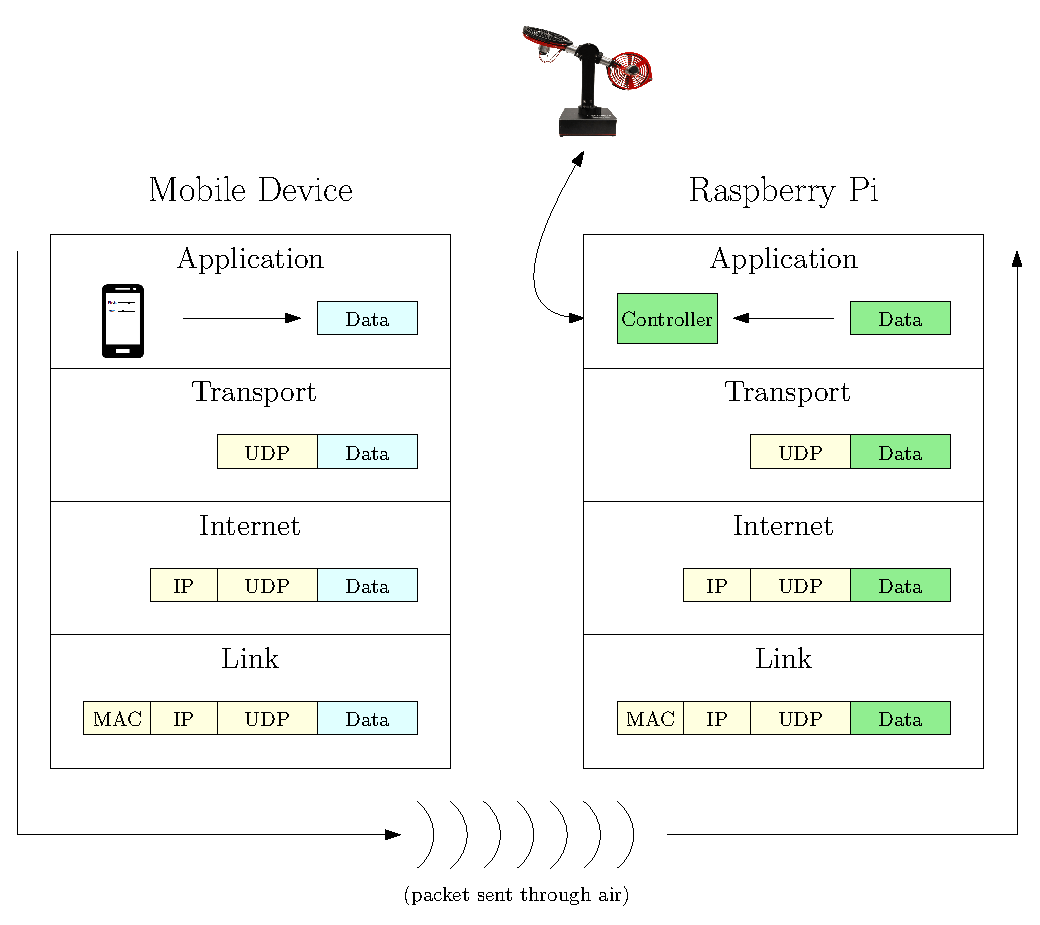
\includegraphics[scale=0.31]{figs/ipe/TCPModel}
  \caption{Communication Model}
  \label{fig:TCPModel}
\end{figure}

\end{frame}

\begin{frame}{Subsystem Level Functional Requirements}{Block Diagram} %Glenn

\begin{figure}
  \centering 
  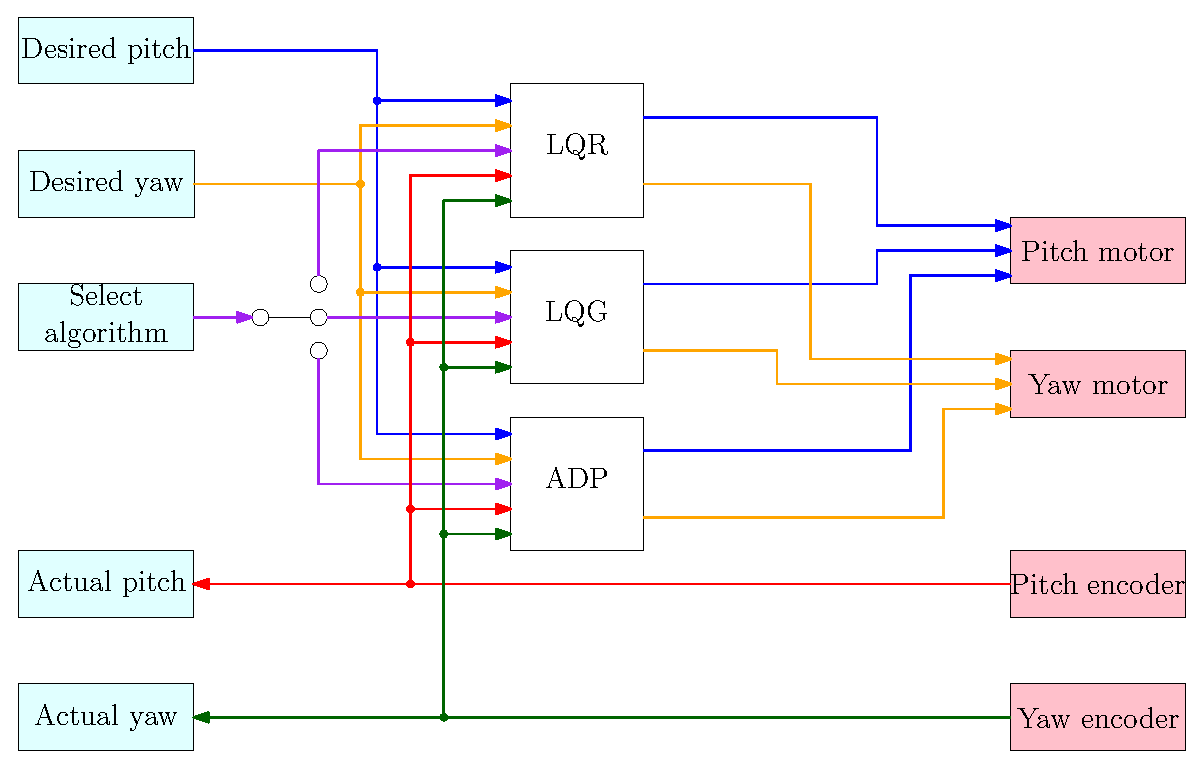
\includegraphics[scale=0.31]{figs/ipe/lowLevel}
  \caption{Low Level Smart Control Diagram}
  \label{fig:lowLevel}
\end{figure}

\end{frame}

%----------------------------------

% \subsection{Specifications}

% \begin{frame}{Subsystem Level Functional Requirements}{Specifications} %Ken
%   The single board computer that will be used is the Raspberry~Pi~3 Model~B:
%     \begin{figure}
%       \centering 
%       \includegraphics[scale=0.35]{figs/raspberry-pi-3-model-b}
%       \caption{Raspberry Pi 3 Model B}
%       \label{fig:raspberry-pi-3-model-b}
%     \end{figure}
% \end{frame}

%----------------------------------

\section{Preliminary Work}

\subsection{LQR Simulation} %Ken

\begin{frame}{Preliminary Work}{LQR Simulation}
    \begin{figure}
      \centering
      \subfigure[][]{
        \label{fig:LQR_Pos_Con}    
        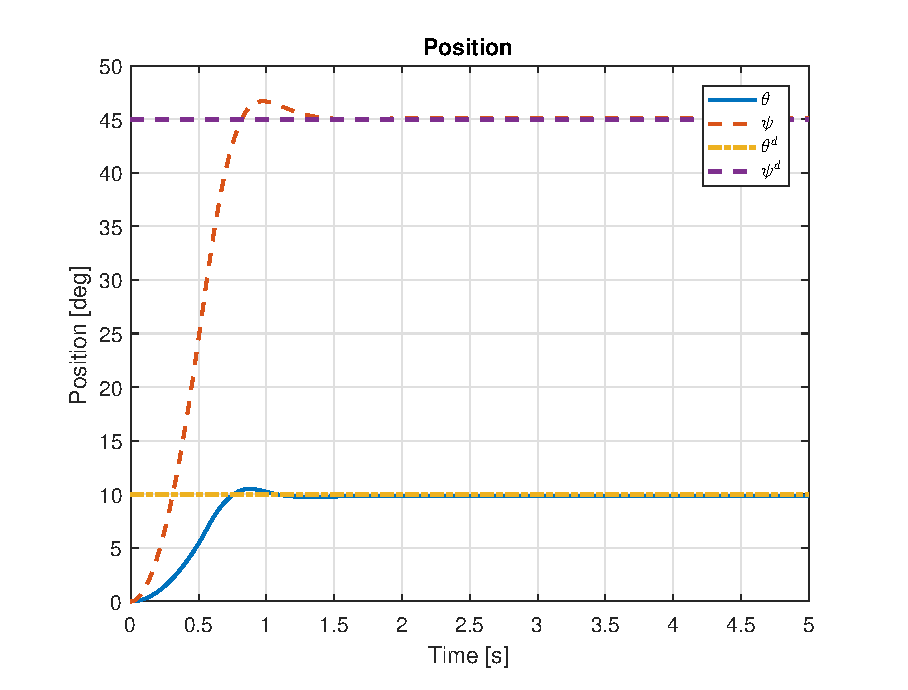
\includegraphics[scale=0.38]{figs/matlab/LQR/P_Simulation/LQR_Pos_Con}
      }
      \subfigure[][]{
        \label{fig:LQR_Volt_Con}
        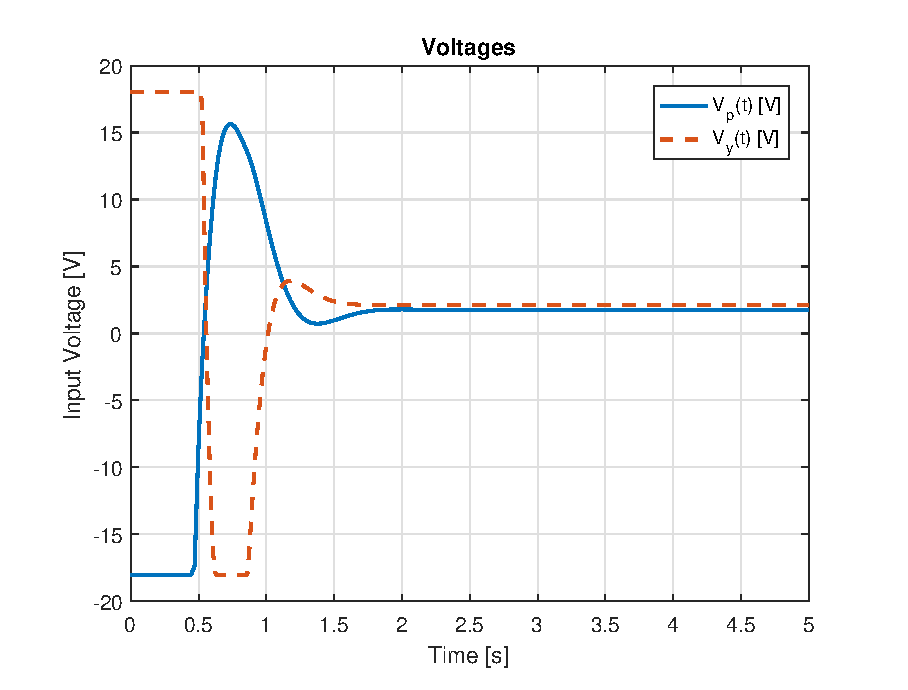
\includegraphics[scale=0.38]{figs/matlab/LQR/P_Simulation/LQR_Volt_Con}    
      }  
      \caption{LQR Simulation \subref{fig:LQR_Pos_Con}~Position and~\subref{fig:LQR_Volt_Con}~Voltage w/ Constant Signal}
      \label{fig:LQR_Sim_Con}
    \end{figure}
\end{frame}

\begin{frame}{Preliminary Work}{LQR Simulation}
    \begin{figure}
      \centering 
      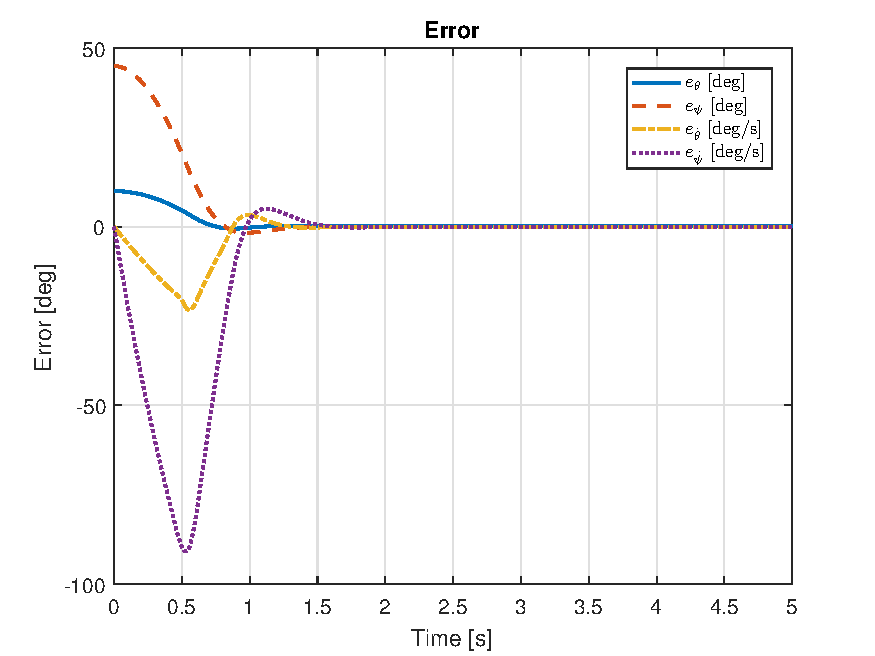
\includegraphics[scale=0.5]{figs/matlab/LQR/P_Simulation/LQR_Error_Con}
      \caption{LQR Simulation Error w/ Constant Signal}
      \label{fig:LQR_Error_Con}
    \end{figure}
\end{frame}


%----------------------------------

\subsection{LQR via USB} %Glenn

% \begin{frame}{Preliminary Work}{LQR via USB}
% \begin{figure}
%       \centering 
%       \includegraphics[scale=0.5]{figs/MATLAB/LQR/USB_results/Pitch_Pos_LQR_USB_SQU}
%       \caption{LQR Pitch Position on PC with Square Wave Input}
%       \label{fig:Pitch_Pos_LQR_USB_SQU}
%     \end{figure}
% \end{frame}

% \begin{frame}{Preliminary Work}{LQR via USB}
% \begin{figure}
%       \centering 
%       \includegraphics[scale=0.5]{figs/MATLAB/LQR/USB_results/Pitch_Volt_LQR_USB_SQU}
%       \caption{LQR Pitch Voltage on PC with Square Wave Input}
%       \label{fig:Pitch_Volt_LQR_USB_SQU}
%     \end{figure}
% \end{frame}

\begin{frame}{Preliminary Work}{LQR via USB}
    \begin{figure}
      \centering
      \subfigure[][]{
        \label{fig:Pitch_Pos_LQR_USB_SQU}    
        \includegraphics[scale=0.38]{figs/matlab/LQR/P_USB/Pitch_Pos_LQR_USB_SQU}
      }
      \subfigure[][]{
        \label{fig:Pitch_Volt_LQR_USB_SQU}
        \includegraphics[scale=0.38]{figs/matlab/LQR/P_USB/Pitch_Volt_LQR_USB_SQU}    
      }  
      \caption{LQR Pitch Position~\subref{fig:Pitch_Pos_LQR_USB_SQU}~and~Voltage~\subref{fig:Pitch_Volt_LQR_USB_SQU} on PC with Square Wave Input}
      \label{fig:Pitch_LQR_USB_SQU}
    \end{figure}
\end{frame}

% \begin{frame}{Preliminary Work}{LQR via USB}
% \begin{figure}
%       \centering 
%       \includegraphics[scale=0.5]{figs/MATLAB/LQR/USB_results/Yaw_Pos_LQR_USB_SQU}
%       \caption{LQR Yaw Position on PC with Square Wave Input}
%       \label{fig:Yaw_Pos_LQR_USB_SQU}
%     \end{figure}
% \end{frame}

% \begin{frame}{Preliminary Work}{LQR via USB}
% \begin{figure}
%       \centering 
%       \includegraphics[scale=0.5]{figs/MATLAB/LQR/USB_results/Yaw_Volt_LQR_USB_SQU}
%       \caption{LQR Yaw Voltage on PC with Square Wave Input}
%       \label{fig:Yaw_Volt_LQR_USB_SQU}
%     \end{figure}
% \end{frame}
\begin{frame}{Preliminary Work}{LQR via USB}
    \begin{figure}
      \centering
      \subfigure[][]{
        \label{fig:Yaw_Pos_LQR_USB_SQU}    
        \includegraphics[scale=0.38]{figs/matlab/LQR/P_USB/Yaw_Pos_LQR_USB_SQU}
      }
      \subfigure[][]{
        \label{fig:Yaw_Volt_LQR_USB_SQU}
        \includegraphics[scale=0.38]{figs/matlab/LQR/P_USB/Yaw_Volt_LQR_USB_SQU}    
      }  
      \caption{LQR Yaw Position~\subref{fig:Yaw_Pos_LQR_USB_SQU}~and~Voltage~\subref{fig:Yaw_Volt_LQR_USB_SQU} on PC with Square Wave Input}
      \label{fig:Yaw_LQR_USB_SQU}
    \end{figure}
\end{frame}


%----------------------------------

\subsection{LQR via Wireless}

\begin{frame}{Preliminary Work}{LQR via Wireless} %Glenn
  %\todo[inline]{Image of the pitch and yaw positions \& voltage will be included in this section for the final presentation}
    \begin{figure}
      \centering
      \subfigure[][]{
        \label{fig:LQR_Pitchpos}    
        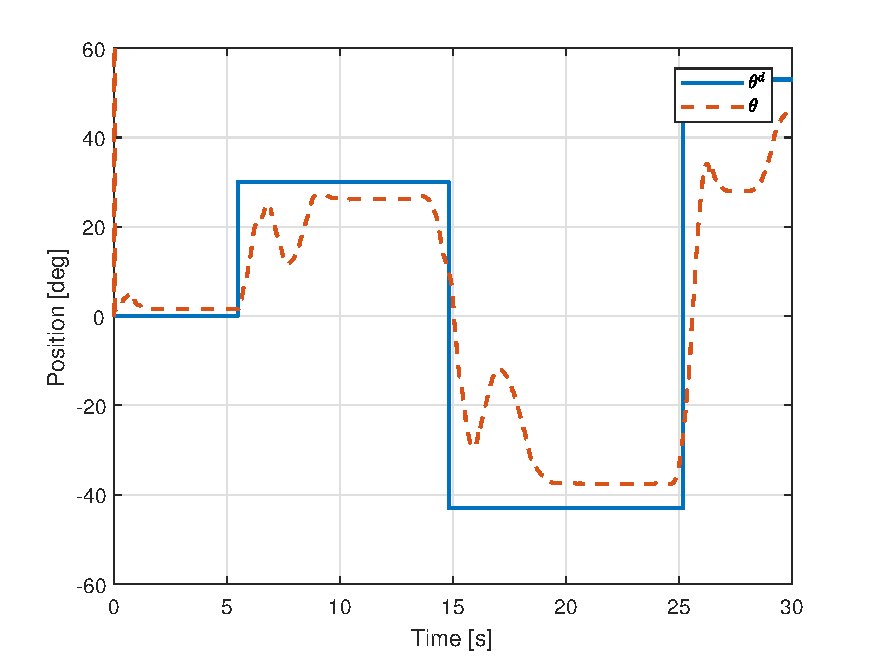
\includegraphics[scale=0.38]{figs/matlab/LQR/P_Android/LQR_Pitchpos}
      }
      \subfigure[][]{
        \label{fig:LQR_PitchVolt}
        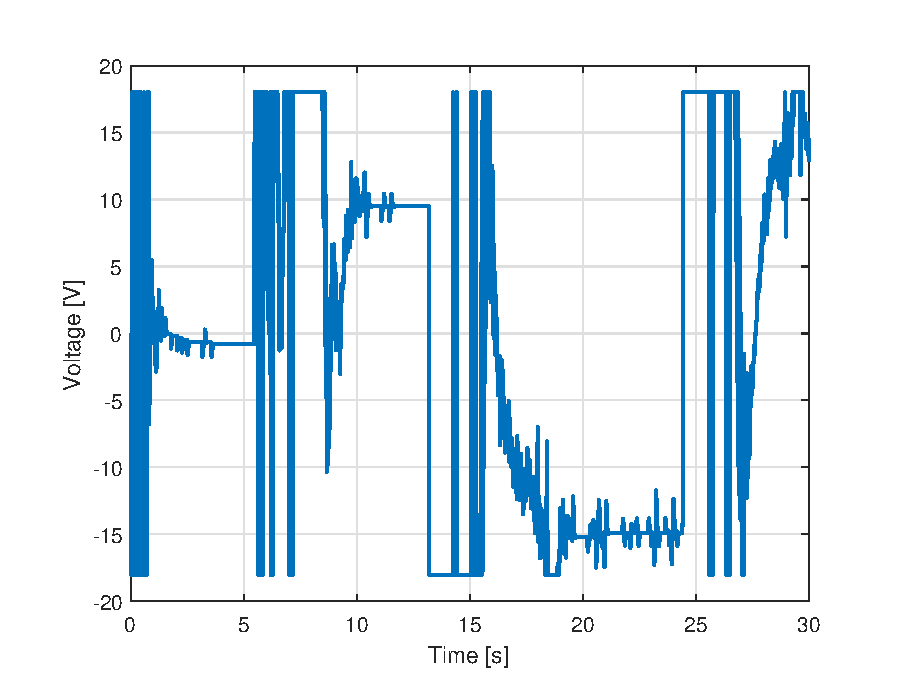
\includegraphics[scale=0.38]{figs/matlab/LQR/P_Android/LQR_PitchVolt}    
      }  
      \caption{Performance in following user's command~\subref{fig:LQR_Pitchpos} tracking pitch angle,~and~\subref{fig:LQR_PitchVolt} pitch motor input voltage}
      \label{fig:performancePitchConst}
    \end{figure}
\end{frame}

\begin{frame}{Preliminary Work}{LQR via Wireless}
    \begin{figure}
      \centering
      \subfigure[][]{
        \label{fig:LQR_Yawpos}    
        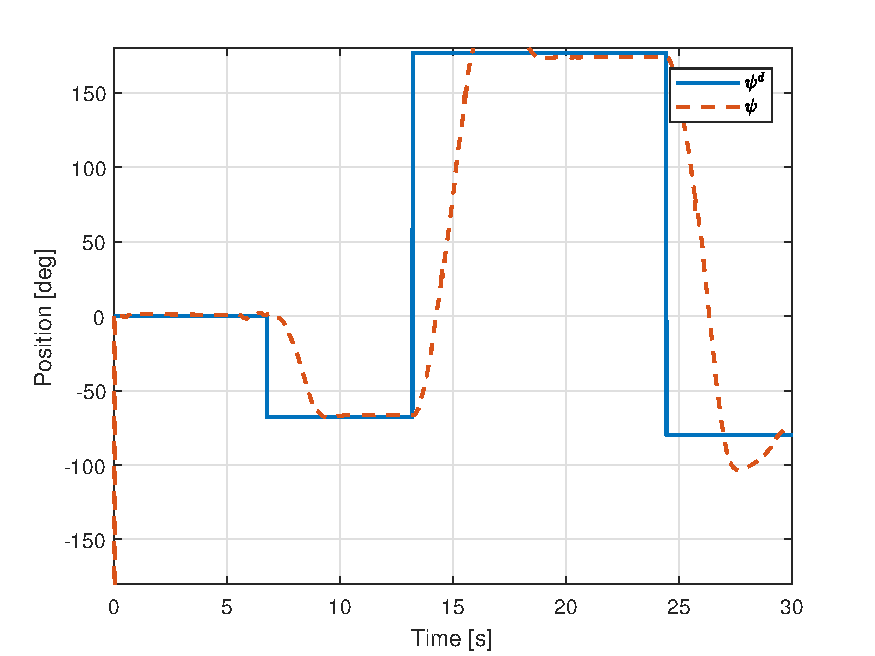
\includegraphics[scale=0.38]{figs/matlab/LQR/P_Android/LQR_Yawpos}
      }
      \subfigure[][]{
        \label{fig:LQR_YawVolt}
        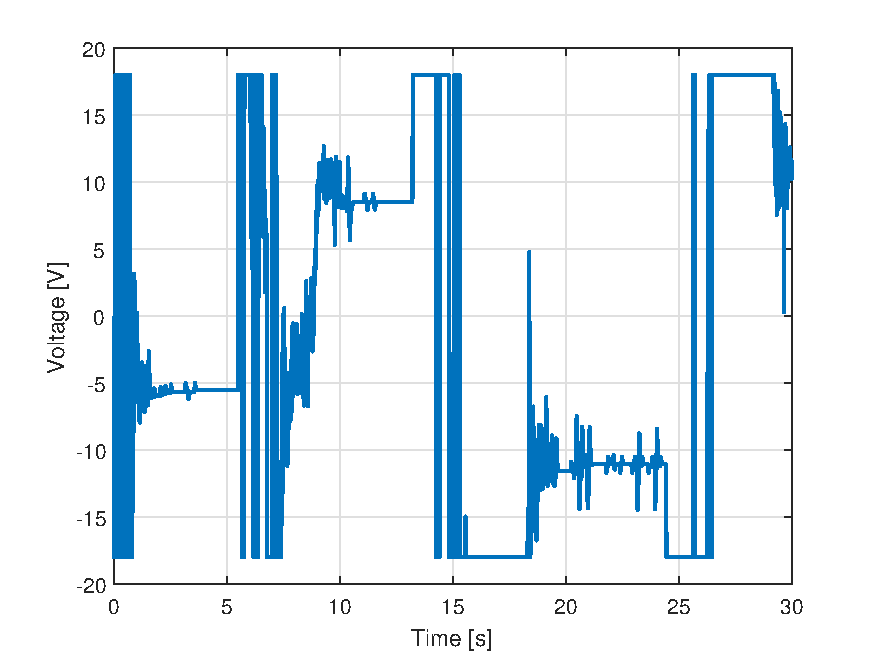
\includegraphics[scale=0.38]{figs/matlab/LQR/P_Android/LQR_YawVolt}    
      }  
      \caption{Performance in following user's command~\subref{fig:LQR_Yawpos} tracking yaw angle,~and~\subref{fig:LQR_YawVolt} yaw motor input voltage.}
      \label{fig:performanceYawConst}
    \end{figure}
\end{frame}

%----------------------------------

\subsection{Demonstration}

\begin{frame}{Demonstration} %Glenn
    %\todo[inline]{A video demonstration the mobile app will be place in this slide}
    \centering
    \includemedia[
     width=0.8\linewidth,
     height=0.6\linewidth,
     activate=pageopen,  
     addresource=videos/Demonstration_Trim.mp4,
     flashvars={
      source=videos/Demonstration_Trim.mp4
      &loop=true  % loop the video
     }
    ]{}{VPlayer.swf}
\end{frame}

%----------------------------------

\section{Parts List}

\begin{frame}{Parts List}{} %Glenn

  \begin{itemize}
      \item Hardware
      \begin{itemize}
        \item Two Quanser Aeros
            \begin{itemize}
                \item Q-flex2 Embedded Panel
            \end{itemize}
        \item Two Single Board Computers (Raspberry Pi 3 Model B)
        \item Android Smart-phone or Tablet\\
        (Note that Apple devices could also be used, however modifications are needed)
      \end{itemize}
      \item Software
      \begin{itemize}
          \item MATLAB \& Simulink
          \begin{itemize}
            \item Raspberry Pi Support Package
            \item Android Support Package
          \end{itemize}
          \item Quanser Real-Time Control (QUARC)
          % "Quanser’s QUARC™ software adds powerful tools and capabilities to Simulink® that make the development and deployment of sophisticated real-time mechatronics and control applications easier. QUARC™ generates real-time code directly from Simulink-designed controllers and runs it in real-time on the Windows target – all without digital signal processing or without writing a single line of code."
      \end{itemize}
  \end{itemize}
\end{frame}

%----------------------------------

%\section{ECE 499 Deliverables}
%\section{Deliverables}

% \subsection{Division of Labor}

% \begin{frame}{Deliverables}{Division of Labor}
%     \begin{columns}
%     \begin{column}{0.5\textwidth}
%         \begin{center}
%             \textbf{Glenn}
%         \end{center}
%         \begin{itemize}
%             \item one
%             \item two
%             \item three
%         \end{itemize}
%     \end{column}
%     \begin{column}{0.5\textwidth}
%         \begin{center}
%             \textbf{Ken}
%         \end{center}
%         \begin{itemize}
%             \item one
%             \item two
%             \item three
%         \end{itemize}
%     \end{column}
%     \end{columns}
% \end{frame}

%----------------------------------

%\subsection{Schedule for Completion}
\section{Schedule for Completion}
\begin{frame}{Deliverables}{Schedule for Completion} %Glenn
   \begin{figure}
    \centering
    \begin{ganttchart}[hgrid,vgrid,x unit=.45cm, y unit title=.5cm,y unit chart=.3cm,milestone label font=\tiny,bar label font=\tiny, group label font=\small,bar/.append style={fill=green},bar incomplete/.append style={fill=red}]{1}{16}
    \gantttitle{2018}{16}\\
    \gantttitle{Sep}{4}
    \gantttitle{Oct}{4}
    \gantttitle{Nov}{4}
    \gantttitle{Dec}{4}\\
    \ganttgroup[progress = 66,group progress label font = \tiny,progress label text={$\displaystyle#1\%$},group progress label anchor = east]{Research}{1}{14} \\
    \ganttbar[progress = 100,progress label text={$\displaystyle#1\%$},bar progress label font = \tiny,bar progress label anchor = east]{Last Years Work}{1}{2}\\
    \ganttbar[progress = 100,bar progress label font = \tiny,progress label text={$\displaystyle#1\%$},bar progress label anchor = east]{LQG}{3}{8}\\
    \ganttbar[progress = 0,bar progress label font = \tiny,progress label text={$\displaystyle#1\%$},bar progress label anchor = east]{ADP}{9}{14}\\
    \ganttgroup[progress = 66,group progress label font = \tiny,progress label text={$\displaystyle#1\%$},group progress label anchor = east]{Simulation}{1}{14}\\
    \ganttbar[progress = 100,bar progress label font = \tiny,progress label text={$\displaystyle#1\%$},bar progress label anchor = east]{LQR}{1}{2}\\
    \ganttbar[progress = 100,bar progress label font = \tiny,progress label text={$\displaystyle#1\%$},bar progress label anchor = east]{LQG}{3}{8}\\
    \ganttbar[progress = 0,bar progress label font = \tiny,progress label text={$\displaystyle#1\%$},bar progress label anchor = east]{ADP}{9}{14}\\
    \ganttgroup[progress = 50,group progress label font = \tiny,progress label text={$\displaystyle#1\%$},group progress label anchor = east]{Implementation}{3}{14}\\
    \ganttbar[progress = 100,bar progress label font = \tiny,progress label text={$\displaystyle#1\%$},bar progress label anchor = east]{LQR USB}{3}{4}\\
    \ganttbar[progress = 100,bar progress label font = \tiny,progress label text={$\displaystyle#1\%$},bar progress label anchor = east]{LQR Raspberry Pi}{5}{6}\\
    \ganttbar[progress = 100,bar progress label font = \tiny,progress label text={$\displaystyle#1\%$},bar progress label anchor = east]{LQR Android}{7}{8}\\
    \ganttbar[progress = 0,bar progress label font = \tiny,progress label text={$\displaystyle#1\%$},bar progress label anchor = east]{LQG USB}{9}{10}\\
    \ganttbar[progress = 0,bar progress label font = \tiny,progress label text={$\displaystyle#1\%$},bar progress label anchor = east]{LQG Raspberry Pi}{11}{12}\\
    \ganttbar[progress = 0,bar progress label font = \tiny,progress label text={$\displaystyle#1\%$},bar progress label anchor = east]{LQG Android}{13}{14}
    \end{ganttchart}
    \caption{Gantt chart for Fall 2018}
    \label{fig:gantt1}
    \end{figure}
\end{frame}

\begin{frame}{Deliverables}{Schedule for Completion}
 \begin{figure}
\centering
\begin{ganttchart}[hgrid,vgrid,x unit=.4cm, y unit title=.5cm,y unit chart=.4cm,milestone label font=\tiny,bar label font=\tiny, group label font=\small,bar/.append style={fill=green},bar incomplete/.append style={fill=red}]{1}{18}
\gantttitle{2019}{18}\\
\gantttitle{Jan}{4}
\gantttitle{Feb}{4}
\gantttitle{Mar}{4}
\gantttitle{Apr}{4}
\gantttitle{May}{2}\\
\ganttgroup[progress = 0,group progress label font = \tiny,progress label text={$\displaystyle#1\%$}, group progress label anchor = east]{Implementation}{3}{8}\\
\ganttbar[progress = 0,bar progress label font = \tiny,progress label text={$\displaystyle#1\%$},bar progress label anchor = east]{ADP USB}{3}{4}\\
\ganttbar[progress = 0,bar progress label font = \tiny,progress label text={$\displaystyle#1\%$},bar progress label anchor = east]{ADP Raspberry Pi}{5}{6}\\
\ganttbar[progress = 0,bar progress label font = \tiny,progress label text={$\displaystyle#1\%$},bar progress label anchor = east]{ADP Android}{7}{8}\\
\ganttgroup[progress = 0,group progress label font = \tiny,progress label text={$\displaystyle#1\%$}, group progress label anchor = east]{Testing}{9}{16}
\end{ganttchart}
\caption{Gantt Chart for Spring 2019}
\label{fig:gantt2}
\end{figure}
\end{frame}

%----------------------------------

% \section{Discussion}

% \begin{frame}{Discussion}{}
  
% \end{frame}

%----------------------------------

\section{Future Directions}

\begin{frame}{Future Directions}{} %Glenn
  \begin{itemize}
    \item Two more motion control algorithms (LQG \& ADP)
    \item Test plan
    \item Implmentation on 6-DOF Helicopter
  \end{itemize}
\end{frame}

% You can reveal the parts of a slide one at a time
% with the \pause command:
%\begin{frame}{Second Slide Title}
%  \begin{itemize}
%  \item {
%    First item.
%    \pause % The slide will pause after showing the first item
%  }
  %\item {   
  %  Second item.
 % }
  % You can also specify when the content should appear
  % by using <n->:
 % \item<3-> {
 %   Third item.
 % }
%  \item<4-> {
%    Fourth item.
 % }
  % or you can use the \uncover command to reveal general
  % content (not just \items):
%  \item<5-> {
%    Fifth item. \uncover<6->{Extra text in the fifth item.}
%  }
%  \end{itemize}
%\end{frame}

%\section{Second Main Section}

% \subsection{Another Subsection}

% \begin{frame}{Blocks}
% \begin{block}{Block Title}
% You can also highlight sections of your %presentation in a block, with it's own %title
% \end{block}
% \begin{theorem}
% There are separate environments for %theorems, examples, definitions and proofs.
% \end{theorem}
% \begin{example}
% Here is an example of an example block.
% \end{example}
% \end{frame}

% Placing a * after \section means it will not show in the
% outline or table of contents.
\section*{Summary}
\begin{frame}{Summary} %Glenn
  \begin{itemize}
    \item Embedded implementation of control algorithms
    \item Mobile interface
  \end{itemize}
  
%   \begin{itemize}
%   \item Outlook
%     \begin{itemize}
%     \item Implementation using two more motion control algorithms (LQG \& ADP)
%     \item Development of a test plan to compare algorithms
%     \end{itemize}
%   \end{itemize}
\end{frame}
% \begin{frame}{Summary}
%   \begin{itemize}
%   \item
%     The \alert{first main message} of your talk in one or two lines.
%   \item
%     The \alert{second main message} of your talk in one or two lines.
%   \item
%     Perhaps a \alert{third message}, but not more than that.
%   \end{itemize}
  
%   \begin{itemize}
%   \item
%     Outlook
%     \begin{itemize}
%     \item
%       Something you haven't solved.
%     \item
%       Something else you haven't solved.
%     \end{itemize}
%   \end{itemize}
% \end{frame}



% All of the following is optional and typically not needed. 
\appendix
\section<presentation>*{\appendixname}
\subsection<presentation>*{For Further Reading}

\begin{frame}[allowframebreaks]
  \frametitle<presentation>{For Further Reading}
  \bibliographystyle{IEEEtran}
  \bibliography{bib/references.bib,bib/refsHelicopter.bib,bib/refsSuruzWeb.bib}
  
%   \begin{thebibliography}{10}
    
%   \beamertemplatebookbibitems
%   % Start with overview books.
    
    
%   \beamertemplatearticlebibitems
 
%   % Followed by interesting articles. Keep the list short. 
    
%     \bibitem{Article1}
% M. Hernandez-Gonzalez, A.Y. Alanis, E.A. Hernandez-Vargas,
% \emph{Decentralized discrete-time neural control for a Quanser 2-DOF helicopter }.
% 2012

% \bibitem{Article2}
% F. Dos Santos Barbosa,
% \emph{4DOF quadcopter: development, modeling and control }.
% 2017

% \bibitem{Article3}
% G.G. Neto, F.S. Barbosa, B.A. Ang\'{e}lico,
% \emph{2-DOF helicopter controlling by pole-placements }.

% \bibitem{Article4}
% Weinan Gao and Zhong-Ping Jiang
% \emph{Data-driven Adaptive Optimal Output-feedback Control of a 2-DOF Helicopter }.

% \bibitem{Article5}
% P. Méndez-Monroy, H. Benítez-Pérez,
% \emph{Fuzzy Control with Estimated Variable Sampling Period for Non-Linear Networked Control Systems: 2-DOF Helicopter as Case Study }. 
% Transactions of the Institute of Measurement \& Control 34, no. 7 (October 15, 2012): 802–14. 
    
%     \bibitem{Article6}
%     Q. Ahmed and A.I.Bhatti and S.Iqbal and I.H. Kazmi
%     \emph{2-Sliding Mode Based Robust Control for 2-DOF Helicopter}.
    
% %   \bibitem{Someone2000}
% %     S.~Someone.
% %     \newblock On this and that.
% %     \newblock {\em Journal of This and That}, 2(1):50--100,
% %     2000.
%   \end{thebibliography}
\end{frame}

\end{document}



%%% Local Variables:
%%% mode: latex
%%% TeX-master: t
%%% End:
